\section{Schema Generation}
\label{sec:stage2}
% ============================================================

Once the textual domain description is distilled into robust, isolated clusters of atomic facts, the pipeline must translate them into a unified relational schema. Bridging the gap between natural language constraints and strict relational algebra in a single step forces an LLM to simultaneously reason about domain semantics and mechanical database normalization. This routinely causes hallucinated keys, dropped requirements, and structurally malformed outputs. 

To systematically decouple these concerns, Schema Generation employs a parallel \emph{shard-and-merge} architecture (Figure~\ref{fig:stage2}). The process first elevates each fact cluster into a localized conceptual model, bypassing rigid relational rules. These conceptual shards are then merged globally using a deterministic mathematical engine that flags contradictions for targeted agentic adjudication. Only when the global conceptual model is perfectly consistent is it mapped deterministically into a SQL-compliant relational schema, which is subjected to a final utility audit.

\begin{figure}[t]
  \centering
  \includegraphics[width=\columnwidth,page=2]{ScribbleDB Image.pdf}
  \caption{The Schema Generation stage. Independent fact clusters are transformed into conceptual shards via a dual-guard repair loop. Shards are deterministically merged, with conflicts resolved by an Adjudicator. The unified conceptual model is mechanically mapped to a relational schema and audited by a Certifier.}
  \label{fig:stage2}
\end{figure}

\subsection{Parallel Conceptual Modelling}
\label{subsec:conceptual-shard}

The input to this phase is the set of independent fact clusters produced in Stage 1. Because these clusters are structurally isolated by design, they can be processed in parallel. For each cluster, an \textsc{ER Extractor} agent is tasked with generating a local Entity-Relationship (ER) shard comprising entities, attributes, and relationships. By restricting the LLM to a purely conceptual vocabulary—omitting foreign keys, indexing, and data types—the model is forced to focus strictly on domain semantics rather than implementation details.

To guarantee that the resulting ER shard faithfully reflects its source facts, the extraction runs within a localized \emph{Dual Guard} repair loop (the top box of Figure~\ref{fig:stage2}):
\begin{enumerate}
    \item \textbf{Conceptual Filter (Deterministic):} The draft shard is immediately evaluated by a mechanical filter that enforces strict invariants without invoking the LLM. It verifies that every entity and attribute maps directly to a provided fact ID and that no syntactically malformed relationships exist. If the filter detects an anomaly, it short-circuits the loop, returning a deterministic error trace directly to the extractor.
    \item \textbf{ER Auditor (Semantic):} Once the draft passes the mechanical filter, it is evaluated by an LLM-based auditor. The auditor cross-references the shard against the atomic facts of that cluster to catch semantic omissions—such as dropped logical constraints or hallucinated relationships that the mechanical filter cannot detect. 
\end{enumerate}
If either guard fails, the localized critique is appended to the extractor's prompt for a retry. A conceptual shard only exits this loop when it satisfies both guards, ensuring structural validity and perfect provenance tracking before global merging.

\subsection{Multi-Verse Merging and Conflict Adjudication}
\label{subsec:merge-adjudicate}

While the individual conceptual shards are internally consistent, they often contain redundant or conflicting representations of the same real-world concepts (e.g., one shard defining a \texttt{Customer} entity while another defines a \texttt{Client}).

Rather than relying on an LLM to blindly guess how to merge the entire fragmented domain, the system applies a deterministic mathematical engine to perform \emph{Multi-Verse Correlation Clustering} (Algorithm~\ref{alg:merge}). This \textsc{Merger} systematically compares entities and relationships across all shards, fusing exact matches and structurally identical nodes. Crucially, when the engine detects semantic or structural disagreements (such as differing cardinality rules or naming overlaps), it does not attempt to resolve them. Instead, it pauses the merge and emits explicit \emph{Conflict Flags}.

These tensions form a \emph{Conflict Graph}, where nodes represent conflicting entities and edges denote the contradictions between them. The system extracts the connected components of this graph and dispatches an \textsc{Adjudicator} agent to resolve each isolated sub-graph in parallel. 

The Adjudicator reviews the conflicting structures alongside their original grounding facts and issues structured resolution patches (for example, merging entities, renaming attributes, or resolving cardinality). These patches are deterministically applied to fix the global conceptual model, ensuring that complex conflict resolution is handled selectively and explicitly by the LLM, rather than burying it in a massive generation step.

\begin{algorithm}[t]
\caption{Multi-Verse Correlation Clustering}
\label{alg:merge}
\begin{algorithmic}[1]
  \Require Local conceptual shards $\mathcal{M}_1, \dots, \mathcal{M}_k$
  \Ensure Unified conceptual model $\mathcal{M}_{\text{global}}$, Conflict flags $F$
  
  \State \textbf{Phase 1: Semantic Scoring}
  \State Flatten all entities across all shards into a global pool $\mathcal{E}$
  \State Compute pairwise semantic similarity scores between all cross-shard entities (using embeddings of attributes and grounding facts)
  \State Convert similarities into a probability matrix $\mathbf{P}$ representing the likelihood that two entities are the same concept
  \State Heavily boost $\mathbf{P}_{ij}$ if two cross-shard entities share an exact name
  
  \State \textbf{Phase 2: Global Clustering}
  \State Construct a weighted graph where edge weight $\mathbf{W}_{ij} = \mathbf{P}_{ij} - 0.5$ (positive for likely merges, negative otherwise, and $-\infty$ for intra-shard pairs)
  \State Partition the graph into clusters $C$ by maximizing the sum of within-cluster edge weights (\textsc{Correlation Clustering})
  
  \State \textbf{Phase 3: Tension Flagging}
  \State Initialize conflict flags $F \gets \varnothing$
  \For{each cross-shard entity pair $(i, j)$}
    \If{they strongly wanted to merge ($\mathbf{P}_{ij} > 0.5$) but ended up in different clusters}
      \State Add \texttt{VETOED\_MERGE} flag to $F$
    \ElsIf{they wanted to remain separate ($\mathbf{P}_{ij} < 0.5$) but were dragged into the same cluster}
      \State Add \texttt{FORCED\_MERGE} flag to $F$
    \EndIf
  \EndFor
  
  \State \textbf{Phase 4: Unification and Validation}
  \State Form unified entities by fusing all attributes and source facts within each cluster
  \State Flag \texttt{IDENTIFIER\_DISAGREEMENT} if fused entities specify conflicting primary keys
  \State Overlay all relationships and deduplicate identical edges
  \State Flag \texttt{CARDINALITY\_CONTRADICTION} if duplicate relationships specify conflicting constraints (e.g., 1:N vs. M:N)
  \State Extract \texttt{ATTR\_SYNONYM} and \texttt{CROSS\_CATEGORY} flags via a secondary probabilistic pass over attribute and relationship names
  \State \Return Unified $\mathcal{M}_{\text{global}}$ and flags $F$
\end{algorithmic}
\end{algorithm}

\subsection{Deterministic Mapping and Certification}
\label{subsec:relational-mapping}

Once the global conceptual model is deduplicated and conflict-free, it must be lowered into an executable relational schema. Because the conceptual model is already structurally perfect, this translation does not require an LLM.

Instead, a deterministic \textsc{Relational Mapper} mechanically applies standard database design rules (Algorithm~\ref{alg:map}). Entities are mapped to tables, multi-valued attributes to junction tables, and conceptual relationships to primary and foreign key constraints. This mechanical lowering completely eliminates the hallucinated keys and circular dependencies that plague single-step LLM schema generators.

Finally, the relational schema undergoes a safety audit by a \textsc{Schema Certifier} agent. The Certifier evaluates the schema against the overarching analytical goal and the full set of facts to ensure that all required metrics and reporting queries can be satisfied. If the schema is structurally sound but analytically deficient, the Certifier emits rigid structural patches to append the missing tables or columns, resulting in the definitive global schema.

\begin{algorithm}[t]
\caption{Deterministic Relational Mapping}
\label{alg:map}
\begin{algorithmic}[1]
  \Require Unified conceptual model $\mathcal{M}$ (Entities $E$, Relationships $R$, FDs)
  \Ensure Relational schema $\mathcal{S}$ (Tables, Columns, Constraints)
  \State Initialize $\mathcal{S} \gets \varnothing$
  \For{each entity $e \in E$}
    \State Base columns $\gets$ all scalar attributes of $e$
    \State PK $\gets$ derive from functional dependencies or defined identifiers
    \If{PK is invalid or missing}
      \State Synthesize surrogate integer PK (e.g., \texttt{e\_id})
    \EndIf
    \State Add table $\mathcal{T}_e$ to $\mathcal{S}$
    \For{each multivalued attribute $a$ in $e$}
      \State Add child table $\mathcal{T}_{e,a}$ to $\mathcal{S}$ with FK referencing $\mathcal{T}_e$.PK
    \EndFor
  \EndFor
  \For{each relationship $r \in R$}
    \If{$r$ is M:N or n-ary}
      \State Name junction table via derived noun rules (avoiding verb collisions)
      \State Add junction table with FKs referencing all participant tables
    \ElsIf{$r$ is 1:N}
      \State Add FK column(s) to the child table referencing the parent table
    \ElsIf{$r$ is 1:1}
      \State Add FK to one participant and enforce \texttt{UNIQUE} constraint
    \EndIf
  \EndFor
  \For{each weak entity $e \in E$}
    \State Append owner table's PK to $\mathcal{T}_e$ as a composite PK and FK
  \EndFor
  \State $\mathcal{S} \gets \textsc{NormalizeAndAlign}(\mathcal{S})$ \Comment{Align data types, wire orphans}
  \State Run deterministic repair loop to prune structurally hollow tables
  \State \Return $\mathcal{S}$
\end{algorithmic}
\end{algorithm}
